\documentclass[11pt]{article}
%\geometry{landscape}                % Activate for for rotated page geometry
%\usepackage[parfill]{parskip}    % Activate to begin paragraphs with an empty line rather than an indent
\usepackage{graphicx}
\usepackage{epstopdf}
\usepackage{enumitem}
\usepackage{subcaption}

\title{Cosmic-ray reconstruction efficiency measurement using an external cosmic-ray counter}
\author{Stefano Roberto Soleti}
\date{January 20, 2017}                                           % Activate to display a given date or no date

\begin{document}
\maketitle
\section*{Questions asked during the Collaboration Meeting}
\begin{description}[style=nextline]
  \item[Elena - Do you use an angular cuts to select your events?]
  It is possible to apply an angular cut to our sample in order to increase the purity. However, the increase in the purity applying a cut of 2$^{\circ}$ on the difference between the extrapolated angles and the reconstructed ones ($\Delta\theta$ and $\Delta\phi$) is less than 0.1\% and it has been considered negligible. The histograms of the angular differences and the results of the cut have been added to the Appendix A of the last version of the internal note.
  \item[E - Are you accounting for decays between in the TPC?]
  No, because when we started this analysis the efficiency was not high enough to consider this effect relevant. However, with the last version of the analysis and an overall efficiency of 96.1\%, the effect of muons triggering the MuCS and decaying or being captured before reaching the TPC must be taken into account. The fraction of this kind of events is $(1.0 \pm 0.1)$\% and the value of the efficiency has been corrected accordingly. A detailed study of this effect has been included in section 5.1 of the last version of the internal note.
  \item[Leon - If you make an angular cut, then the scatter plot of points of the MuCS will look nicer?]
  Yes, the effect of the angular cut would be to remove the events with a large scattering of the cosmic muon. Figure \ref{fig:alignment} shows the extrapolated points for the upstream configuration before (\ref{fig:upstream}) and after (\ref{fig:upstream_after}) an angular cut of 5$^{\circ}$ on $\Delta\theta$ and $\Delta\phi$. However, the point of that plot was to show that the majority of the MuCS-tagged tracks can be extrapolated back to the height of the panels.
  \begin{figure}[htbp]
    \begin{subfigure}{0.5\textwidth}
      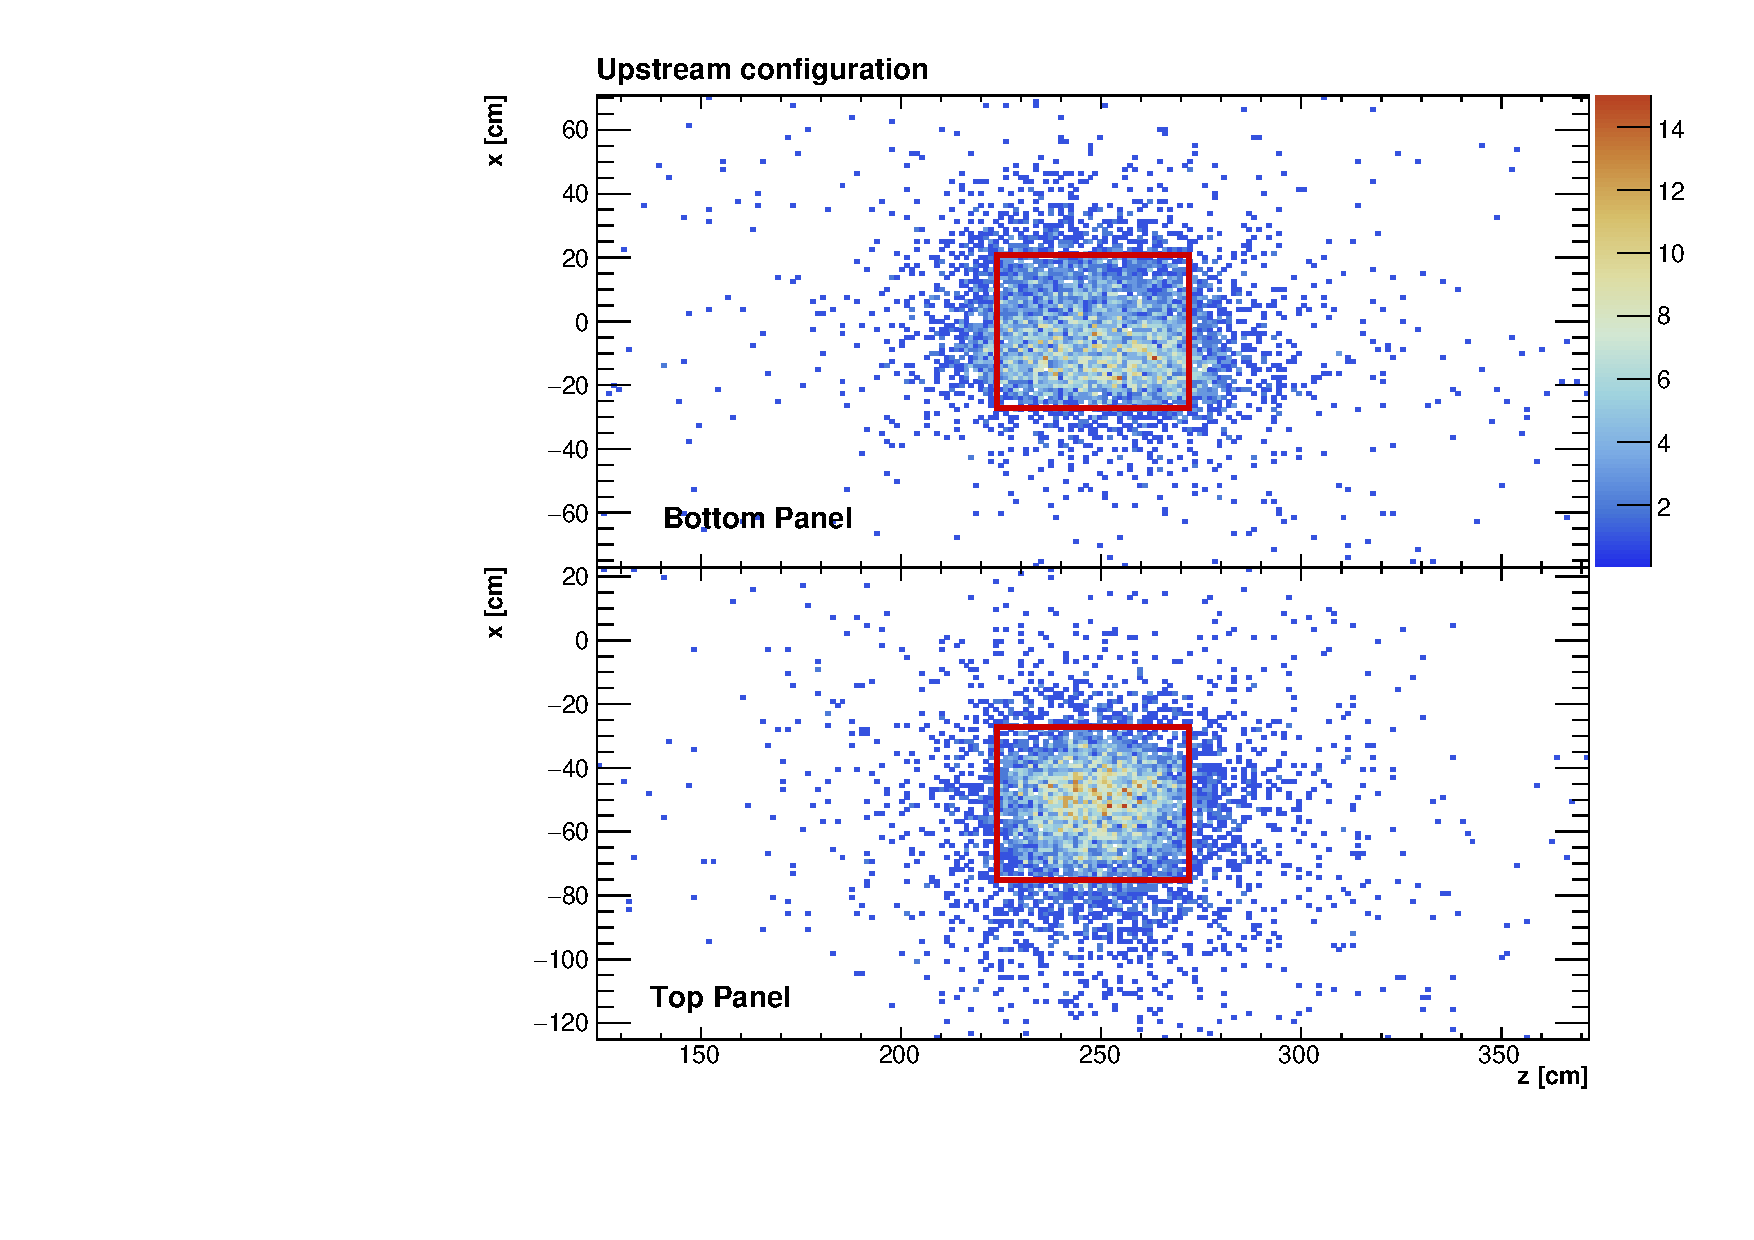
\includegraphics[width=\linewidth]{../figures/upstream.pdf}
      \caption{Upstream - before angular cut} \label{fig:upstream}
    \end{subfigure}
    \begin{subfigure}{0.5\textwidth}
      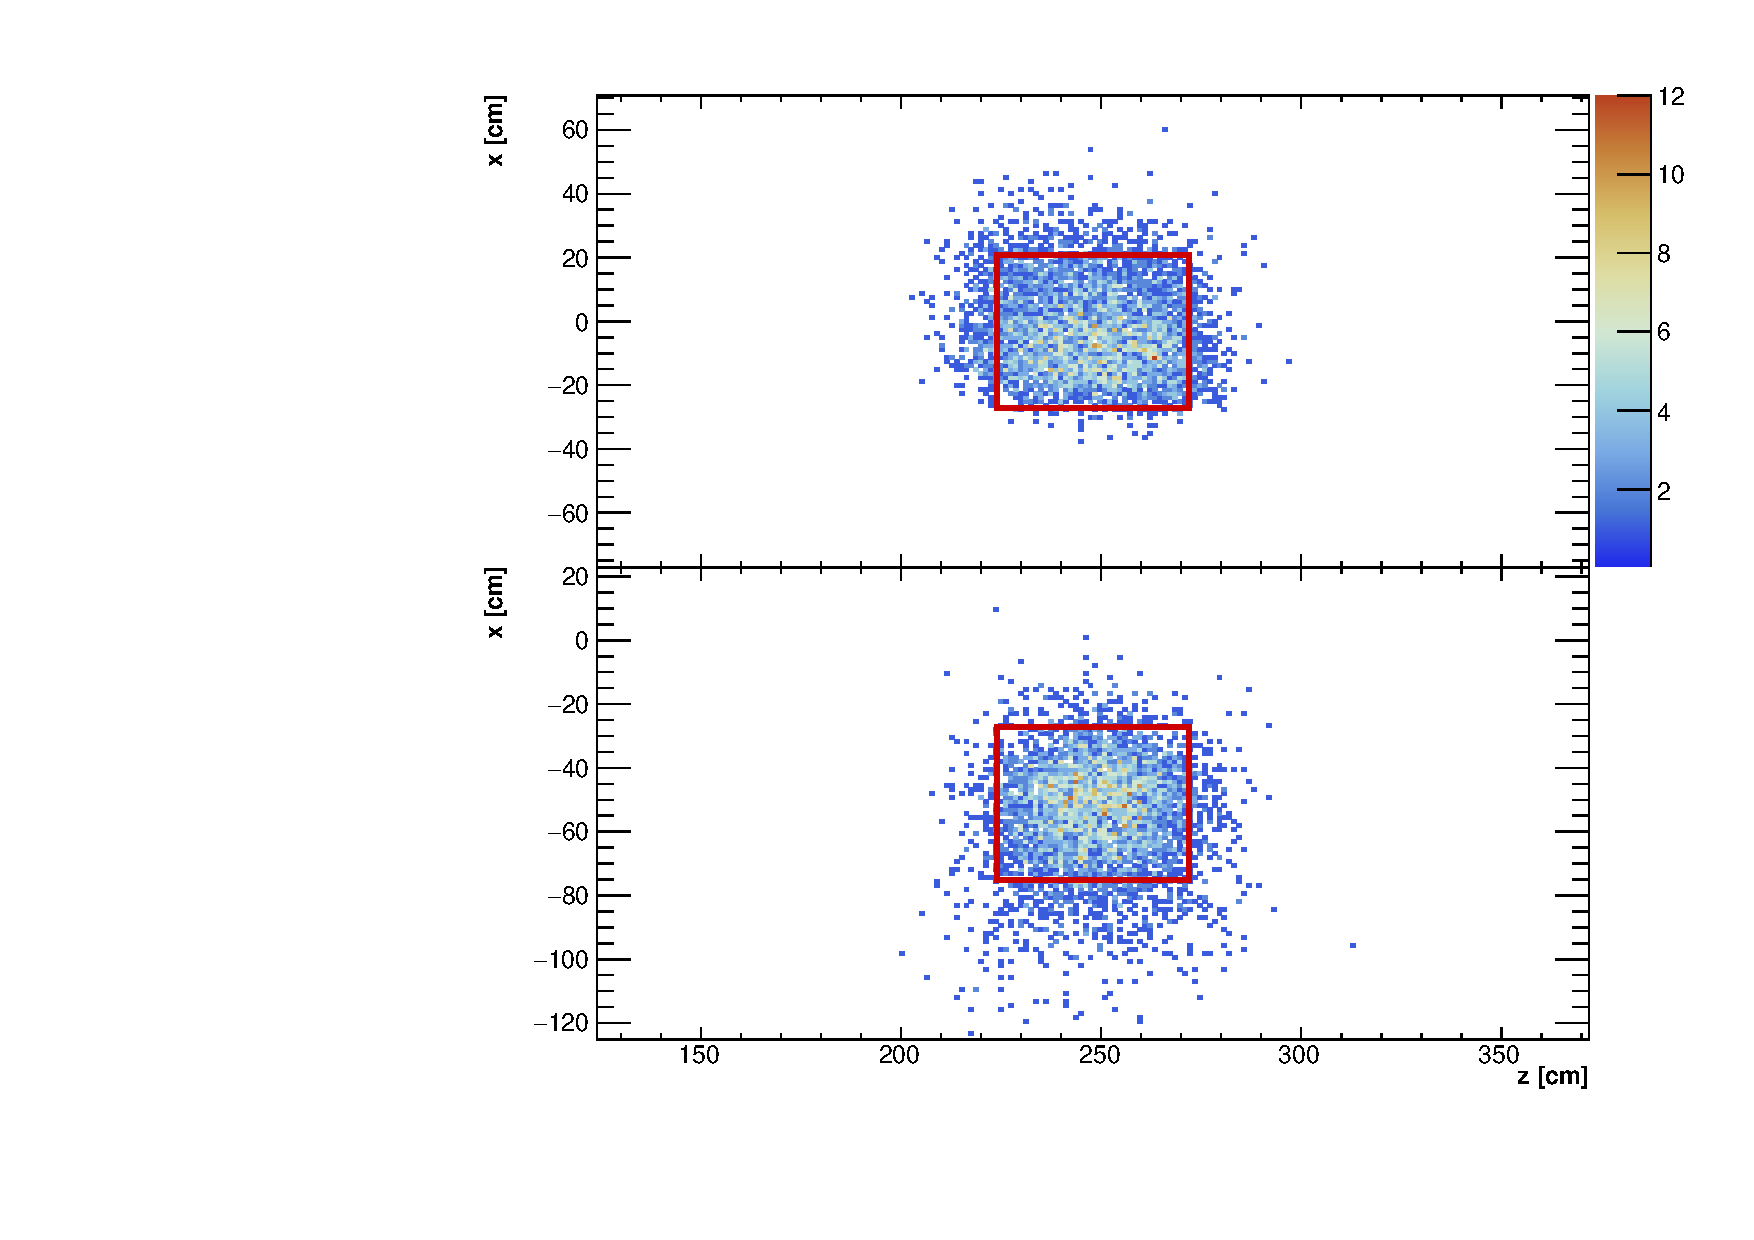
\includegraphics[width=\linewidth]{../figures/upstream_after.pdf}
      \caption{Upstream - after angular cut} \label{fig:upstream_after}
    \end{subfigure}

    \caption{Extrapolated points of the MuCS-tagged tracks at the height of top and bottom panels for the upstream configuration before and after an angular cut of 5$^{\circ}$ on $\Delta_{\theta}$ and $\Delta_{\phi}$.} \label{fig:alignment}
  \end{figure}
  \item[Mike K - How do you reconcile 96.1\% reconstruction efficiency with the few percent efficiency quoted by Tim Bolton?]
  Our efficiency and the one quoted by Tim cannot be compared directly. In our case, we know there must be a cosmic ray in a well-defined area of the detector, while Tim's 6\% refers to CC-inclusive events, whose topology is different and its position in the detector is unknown.
\end{description}

%\subsection{}



\end{document}
